\documentclass[a4paper]{article}

%% Language and font encodings
\usepackage[T1]{fontenc}
\usepackage[utf8x]{inputenc}
\usepackage[english]{babel}

\usepackage[colorlinks=true, allcolors=blue]{hyperref}

\urlstyle{tt}
\newcommand{\email}[1]{\href{mailto:#1}{\tt{\nolinkurl{#1}}}}
\newcommand{\orcid}[1]{ORCID: \href{https://orcid.org/#1}{\tt{\nolinkurl{#1}}}}

\newcommand{\figleg}[1]{\centering\itshape{#1}\/}
\newcommand{\figref}[1]{(see figure~\ref{#1})}

\usepackage[sfdefault,lf]{carlito}
%% The 'lf' option for lining figuressy
%% The 'sfdefault' option to make the base font sans serif
\usepackage[parfill]{parskip}
\renewcommand*\oldstylenums[1]{\carlitoOsF#1}%
\usepackage{fancyhdr}
\usepackage{natbib}
\usepackage{authblk}
\setlength{\headheight}{41pt}

%% Sets page size and margins
\usepackage[a4paper,top=3cm,bottom=2cm,left=3cm,right=3cm,marginparwidth=1.75cm]{geometry}

%% Useful packages
\usepackage{amsmath}
\usepackage{amssymb}
\usepackage{graphicx}
\usepackage{booktabs}
\usepackage{caption}
\usepackage{subcaption}

\usepackage[colorinlistoftodos]{todonotes}

\fancyhead[L]{Posted: \today}
\fancyhead[R]{

\includegraphics[width=4cm]{img/engrXiv_banner.png}
}
\pagestyle{plain}
\title{Adaptive Removal of the Transcranial Alternating Current Stimulation Artifact from the Electroencephalogram}
\author[1,*]{Robert Guggenberger}
\author[1]{N.N.}
\affil[1]{Department for Translational Neurosurgery, University Hospital Tübingen}

\affil[*]{Corresponding author: \email{robert.guggenberger@posteo.eu}}
\date{\today}

\usepackage{varioref}
\usepackage{hyperref}
\usepackage{cleveref}
\hypersetup{hidelinks = true}

\usepackage[nonumberlist,acronym]{glossaries}
% abbreviations:
\newacronym{eeg}{EEG}{electroencephalogram}
\newacronym{tacs}{tACS}{transcranial alternating current stimulation}
\newacronym{tms}{TMS}{transcranial magnetic stimulation}
\newacronym{tpca}{tPCA}{temporal principal component analysis}
\newacronym{sma}{SMA}{superposition of moving averages}
\newacronym{erp}{ERP}{event-related potential}
\makeglossaries{}

% --------------------------------------------------------------------------
\begin{document}
\maketitle
\thispagestyle{fancy}

\begin{abstract}
Your abstract.
\end{abstract}

\section{Introduction}

The combination of \gls{tacs} and \gls{eeg} has been explored in several recent studies. While the analysis of \gls{eeg} before or after stimulation posits limited technical challenges, the \gls{eeg} recording during stimulation is heavily affected by the stimulation artifact.

\subsection{Matched Phase and Frequency}
Computational simulations suggest that the power of endogenous oscillations would increase most if the frequency of~\gls{tacs} matches the targets eigenfrequency~\citep{Kutchko_2013,Zaehle_2010}.
This has been supported by evidence from animal studies~\citep{Schmidt_2014}, and human studies combining \gls{tacs} with \gls{tms} \citep{Guerra_2016}, or contrasting pre and post resting state power analysis \citep{Zaehle_2010}.
It has also been suggested that the phase of neuronal populations would be locked to the phase of the \gls{tacs} signal \citep{Reato_2013}. This has been supported by evidence from studies combining \gls{tacs} with motor output \citep{Brittain_2013}, \gls{tms}~\citep{Raco_2016,Nakazono_2016} or sensory perception~\citep{Gundlach_2016}.

This suggests that the effect of \gls{tacs} can result in neurophysiological effects which are phase-and frequency-matched to the stimulation artifact. Such frequency and phase matching between \gls{tacs} and \gls{eeg} recordings can render the removal of the artifact difficult or impossible, as the signal might no longer be separatable from the artifact.

\subsection{Non-Stationary Amplitude Modulation}

An approach to tackle this issue is to assess the time-course of the~\gls{eeg} signal. Consider the assumption that the artifact is stationary and superpositioned on the physiological signal. Then, modulations in the amplitude of the recorded~\gls{eeg}-signal must be caused by changes in the underlying physiology.
This would be the case, even if frequency and phase are matched to the stimulation signal. Approaches assuming such stationarity of the stimulation artifact have been used e.g.\ by~\cite{Pogosyan_2009}.

Yet, detailed analysis of the stimulation artifact provides evidence that the artifact amplitude is actually not stationary. Instead, the amplitude is modulated by heart-beat and respiration~\citep{Noury_2016}. Recently, non-linearities in how stimulators control the applied current has been suggest as further source of modulation~\citep{Neuling_2017}.
It has been argued that unregularized spatial filters might be able to remove this amplitude modulation~\citep{Neuling_2017}. But if only few channels are recorded, the method can fail, as the estimation of the spatial covariance is insufficient, or impossible in the single-channel-case.
Consider furthermore that event-related responses like modulation of skin impedance can also affect the scalp conductance at stimulation electrodes. This would introduce event-related amplitude modulation of the stimulation artifact. In that regard, disentangling true signal from the stimulation artifact stays technically challenging.

\subsection{Artifact Distortion}

Ideally, the stimulation artifict of~\gls{tacs} resembles a sinusoid. Yet, practical experience suggests that the signal is usually distorted to various degrees.
Figure~\ref{fig:nonsinus} shows examples of distortion and saturation in two recordings of \gls{tacs}-\gls{eeg}. The gray traces indicate nine invididual periods, while the red trace indicates their average. In figure~\ref{fig:distortion}, note the periodic, yet non-sinusoidal waveform. In figure~\ref{fig:saturation}, note the saturation.

\begin{figure}[hbtp]
    \begin{subfigure}{.5\textwidth}
    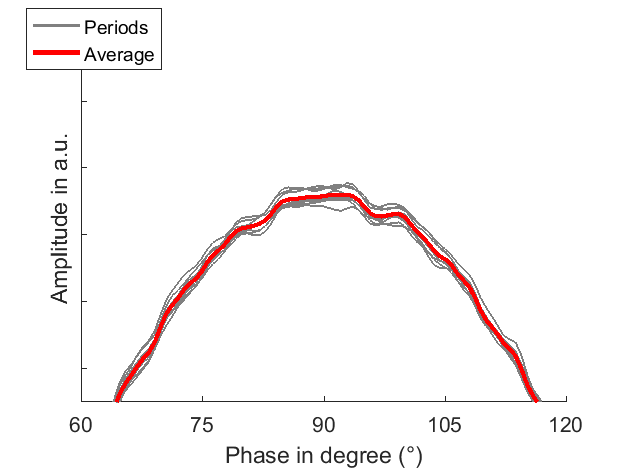
\includegraphics[width=\textwidth]{./img/intro/distortion.png}
    \caption{Distortion}\label{fig:distortion}
    \end{subfigure}
    \begin{subfigure}{.5\textwidth}
    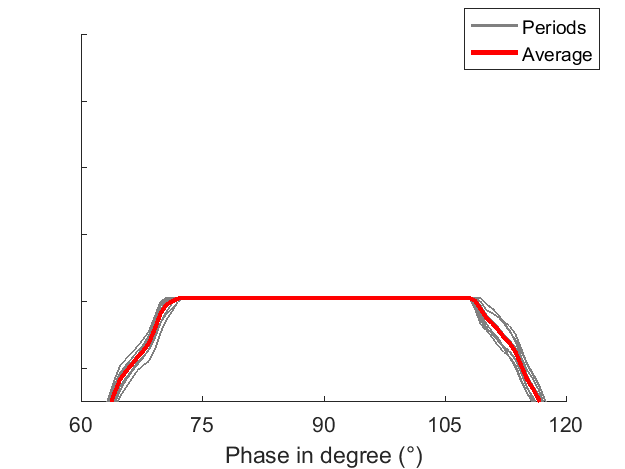
\includegraphics[width=\textwidth]{./img/intro/saturation.png}
    \caption{Saturation}\label{fig:saturation}
    \end{subfigure}
    \caption{Examples for loss of sinusoidal fidelity}\label{fig:nonsinus}
\end{figure}

The temporally and spatially uneven impedance distribution has been suggested as cause of distortion, rendering the resulting waveform periodic, but non-sinusoidal. A major problem is amplifier saturation, i.e.\ the stimulation artifact exhibiting an amplitude to large for the dynamic range of the amplifier, causing the signal to be cut off and information to be lost.
Additionally, non-linearites in the amplifier slew rate can distort the shape even when the signal is close to the saturation threshold.

\subsection{Computational Demands}

Methods based on adaptive template construction and \gls{tpca}~\citep{Niazy_2005} have been explored for removal of  non-stationary and misshaped \gls{tacs} artifacts~\citep{Helfrich_2014}.  Consider that the process of template construction, the estimation of accurate weights for removal by template subtraction and the suqsequent removal of residual artifacts using \gls{tpca} is computationally cumbersome. Additionally, it often requires off-line analysis supported by visual inspection.
Such a multi-staged template-approach is therefore of limited utility for on-line artifact removal. Furthermore, critical evaluation has suggested that the residual artifact spans several principal components, and a sufficient artifact removal is therefore not possible with \gls{tpca} \citep{Noury_2016}.

\subsection{Motivation}

We were interested in development of a computationally fast approach, feasible for online artifact removal. At the same time, the approach was required to account for the dynamical modulation of the artifact amplitude, and the possibility of non-sinusoidal distortion and saturation. Ideally, the approach would allow to derive physiological signals at the frequency of stimulation, even if physiological oscillations were phase-locked to the stimulation signal.

\section{Approach}

The main idea is that at any given time point $t$, the recorded signal $r(t)$ is a linear super\-position of a neurophysiological signal $n(t)$, the stimulation artifact $a(t)$ and a white noise term $e(t)$. The task is to recover $n(t)$ by estimating $\hat{a}(t)$ and $e(t)$ and subtracting from $r(t)$.

\begin{eqnarray}
    r(t) = n(t) + a(t) + \epsilon(t)\\
    n(t) = r(t) - \hat{a} - \epsilon(t)
\end{eqnarray}

\subsection{Periodic Estimation}
Assume that the~\gls{tacs} artifact were \emph{non-sinusoidal}, but \emph{stationary and periodic}. At the same time, assume that neurophysiological signals $n$ and noise $\epsilon$ were absent.
Then, we could estimate the amplitude of $a$ at any time-point $t$ by using the signal $r$ recorded from any time-point, as long as this time-point is an integer multiple of the artifacts period length $p$ earlier~\eqref{eq:Comb}.
Subtraction of a delayed version of the signal is also known as comb filter. Please note that for discretely sampled signals, this approach only works if the frequency of the artifact is an integer divisible of the sampling frequency.

\begin{eqnarray}
    \hat{a}(t) = r(t-np)\label{eq:Comb}\\
    n \in \mathbb{Z}
\end{eqnarray}

\subsubsection{Uniform Comb Filter}

Consider that the noise term $\epsilon$ is still superpositioned on $r$. If the noise term were white, and because the expectation of white noise $\langle\epsilon\rangle$ converges asymptotically to zero with increased sample size, an approach to estimate a bias-free  artifact amplitude would be to average across as many earlier periods as possible~\eqref{eq:Uniform}.
Subsequently, this estimate can be used to  remove the artifact from $r$.
In real applications, stimulation duration is limited and computational constraints exist. This is reflected by the fact that we have to use a finite number for $N$.

\begin{equation}
    \hat{a}(t) = \sum_{n=1}^{N} \frac{r(t - np)}{N}\label{eq:Uniform}
\end{equation}

\subsubsection{Superposition of Moving Averages}

Please note that averaging across neighbouring periods $M$~\eqref{eq:SMA} has been suggested before and termed~\gls{sma} by~\cite{Kohli_2015}.

\begin{equation}
    \hat{a}(t) = \sum_{n-M/2}^{n+M/2} \frac{r(t - np)}{M+1}\label{eq:SMA}
\end{equation}

Consider that the approach using only past values~\eqref{eq:Uniform} returns a causal filter. Applied online, a causal filter would be able to remove the artifact without the delay of $(Mp)/2$ necessary for~\gls{sma}. Furthermore,~\gls{sma} is well-defined only for even $M$. This motivates the exploration of causal filters for artifact removal.

\subsection{Temporal Weighting}

Consider that the amplitude of the  artifact has been described to be non-stationary and dynamically modulated~\citep{Noury_2016,Neuling_2017}.
Although it has been suggested that there are event-dependent components of the amplitude modulation (e.g.\ by heartbeat or respiration~\cite{Noury_2016} or stimulator impedance check~\cite{Neuling_2017}), the parameters of the dynamical system governing event-independent amplitude modulation are usually not known a priori.This can render online artifact removal problematic.

One approach to tackle this problem is to use instead of a constant weight $1/N$~\eqref{eq:Uniform}, a time-dependent weighting function $w_n$~\eqref{eq:Weighted}.
\begin{equation}
    \hat{a}(t) = \sum_{n=1}^{N} w_n r(t - np)\label{eq:Weighted}
\end{equation}

\subsubsection{Justification by Sampling}
Consider for example the simple one-step comb filter, where we remove the artifact by subtracting a value sampled from any earlier period.
Assume now that this value were not drawn from the last period, but instead drawn at random from the last $N$ periods with uniform distribution. If the system governing amplitude modulation were fully stationary for the last $N$ periods, performance would in law be virtually identical to the comb filter based on averaging~\eqref{eq:Uniform}.
If it were instead governed by a random process\footnote{at least for the past time-points $N$}, e.g.\ a Wiener process, the precision of the estimate would be expected to degrade as a function of the delay. This rationale justifies non-uniform weights, and to use weights that are linked to the precision of the sample.

\subsubsection{Justification by AR~(1) process}

Consider that the system governing the amplitude of the stimulation artifact could be decomposed into the constant amplitude $c$ controlled by the stimulator and a dynamical, \emph{event-unrelated} AR~(1) process governing the amplitude modulation. This would return for $N$ approaching infinity:

\begin{align}
    X_{t} = c + \sum_{n=0}^{\infty} \phi_n \epsilon_{t-k}\label{eq:AR1process}
\end{align}
If the kernel $\Phi$  behind the modulation of the artifacts amplitude were known, or could be estimated sufficiently, we could construct an optimal weighting function as a deconvolution filter.
This line of reasoning is based on the similarity between the generic weighted comb filter~\eqref{eq:Weighted} and the generic discrete-time AR~(1) process~\eqref{eq:AR1process}.
Note that, for practical applications, we would need finite $N$. This would limit the application to kernels decaying sufficiently fast.

\subsubsection{Criteria}

If we do not know the generating kernel, we might select a generic weight function with well-known behavior. By controlling the parameters of weight functions, we might better match the process governing the amplitude modulation. This might allow us to achieve a better artifact estimation and subsequent removal.
For example, in the case of the uniform filter, we have a shape parameter $N$, defining how far back we trust a measurement to have the same precision as earlier samples.
The qualifying criteria for these weighting functions are that the sum of all their weights should be equal to one. This keeps the weighting function in agreement with the uniform comb filter~\eqref{eq:Uniform} and returns an unbiased estimate in the case of full stationarity. Additionally, it keeps the filter stable. In the following sections, we will discuss three weighting functions assuming non-skewed and unbiased generating processes.

\subsection{Temporal Weighting Examples}

\subsubsection{Linear Weighting}

One straight-forward approach is using a linear decreasing weighting function. The assumption of local linearity is widely used in the analyis of non-linear dynamical systems, which could render the kernel sufficiently flexible.
Additionally, the function is simple and the necessary normalization can easily be calculated by using the triangular number for a given $N$ as normalizing constant $k$~\eqref{eq:NormLinear}.
Hence, equation~\eqref{eq:Linear} returns weights for earlier periods based on a linear temporal weight decay.

\begin{equation}
    w_n = \frac{N-n+1}{k}\label{eq:Linear}
\end{equation}
with the following normalization
\begin{equation}
    k  = \sum_{n=1}^{n} n = \frac{N(N+1)}{2}\label{eq:NormLinear}
\end{equation}

\subsubsection{Exponential Weighting}

Motivated by the fact that the autocorrelation function of an AR~(1) process can be expressed as a decaying exponential, an alternative approach would be an exponential weighting function. The time constant $\tau$ of an exponential controls its temporal decay. To maintain the shape across different $N$, we consider it reasonable to normalize $n$ by $N$. Hence, equation~\eqref{eq:Exp} returns weights for earlier periods based on their exponential temporal weight decay.

\begin{equation}
    w_n = \frac{1}{k} e^{\tau-\tau{(n/N)}}\label{eq:Exp}
\end{equation}
with the following normalization
\begin{equation}
    k  = \sum_{n=1}^{N} e^{\tau-\tau{(n/N)}}\label{eq:NormExp}
\end{equation}

\subsubsection{Gaussian Weighting}

Consider that the amplitude modulation might be governed by more than one AR~(1) process, or the process might be non-stationary itself.
Motivated by the fact that such sums  often converge to a normal distribution, an alternative approach would be a Gaussian weighting function.
Using a suitable parameterization, and centering on zero, the inverse of the standard deviation $\frac{1}{\sigma^2}$ defines the time constant $\tau$ of a Gaussian distribution, which controls its temporal decay.
To maintain the shape across different $N$, we consider it again reasonable to normalize $n$ by $N$. Hence, equation~\eqref{eq:Gauss} returns weights for earlier periods based on their Gaussian temporal weight decay.

\begin{equation}
    w_n = \frac{1}{k} f(n/N)\label{eq:Gauss}
\end{equation}
with the following generating function and normalization
\begin{align}
    f(x)  & = \sqrt{\frac{\tau}{2\pi}} e^{-(\tau x^2)/2}  \\
    k  & = \sum_{n=1}^{N} f(n/N)\label{eq:NormGauss}
\end{align}


\section{Evaluation}

We implemented functions for kernel creation and artifact removal in Matlab 2016b. Code\footnote{\url{https://github.com/agricolab/ARtACS}}  can be accessed online. We evaluated the behavior of the various kernels regarding their frequency response characteristics~(see~\ref{sec:EvaluationFreq}) as well as their behavior on simulated~(see~\ref{sec:EvaluationSimulated})  and real data~(see~\ref{sec:EvaluationData}).

\subsection{Evaluation of Frequency Response}\label{sec:EvaluationFreq}

\subsubsection{Exemplary Kernels}

Examine the following exemplary kernels constructed for a sampling rate of 1KHz, a stimulation frequency of 10 Hz and a memory of 10~\figref{fig:ExemplaryCausalKernels}.

\begin{figure}[hbtp]
    \begin{subfigure}{.245\textwidth}
        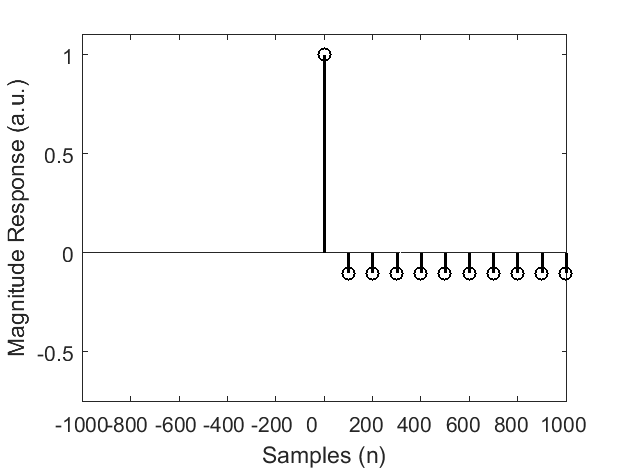
\includegraphics[width=\textwidth]{img/causal/kernel_ave.png}\\
        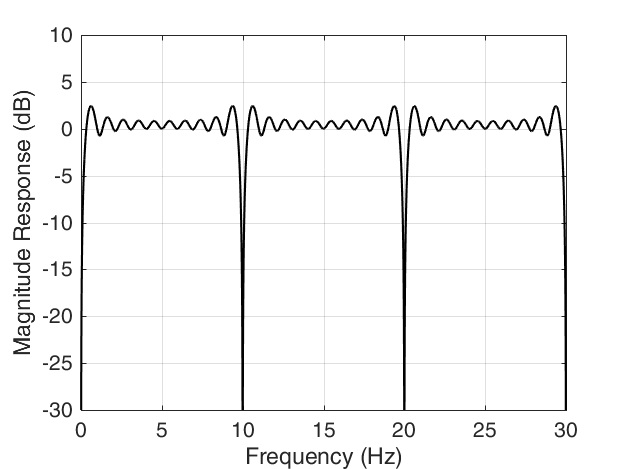
\includegraphics[width=\textwidth]{img/causal/mag_ave.png}
        \caption{Uniform}\label{fig:UniformKernel}
    \end{subfigure}
    \begin{subfigure}{.245\textwidth}
        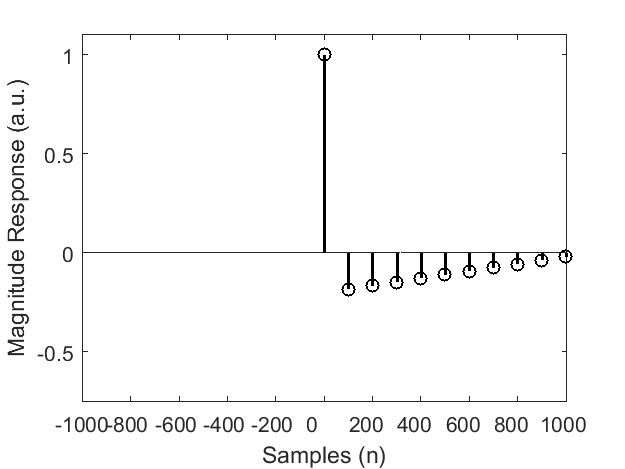
\includegraphics[width=\textwidth]{img/causal/kernel_linear.png}\\
        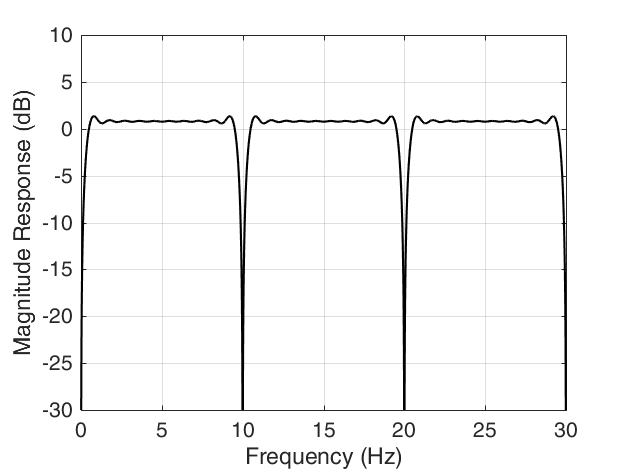
\includegraphics[width=\textwidth]{img/causal/mag_linear.png}
        \caption{Linear}\label{fig:LinearKernel}
    \end{subfigure}
    \begin{subfigure}{.245\textwidth}
        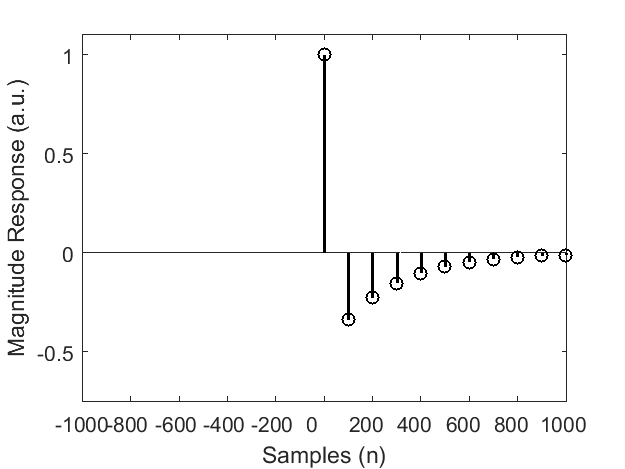
\includegraphics[width=\textwidth]{img/causal/kernel_exp.png}\\
        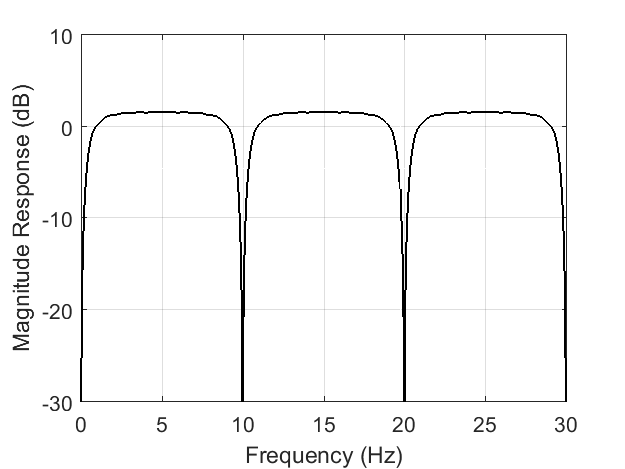
\includegraphics[width=\textwidth]{img/causal/mag_exp.png}
        \caption{Exponential~$\tau=4$}\label{fig:ExponentialKernel}
    \end{subfigure}
    \begin{subfigure}{.245\textwidth}
        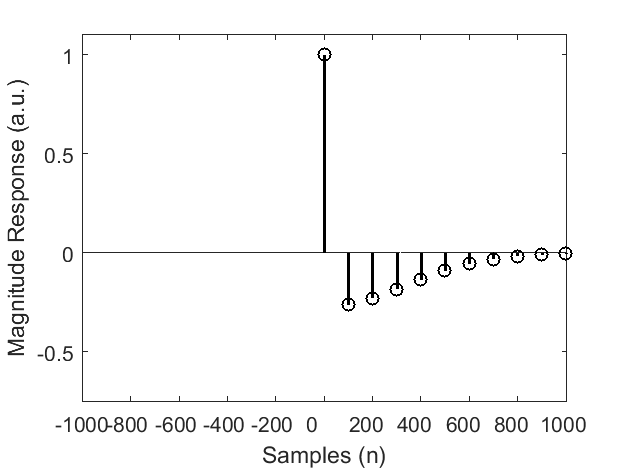
\includegraphics[width=\textwidth]{img/causal/kernel_gauss.png}\\
        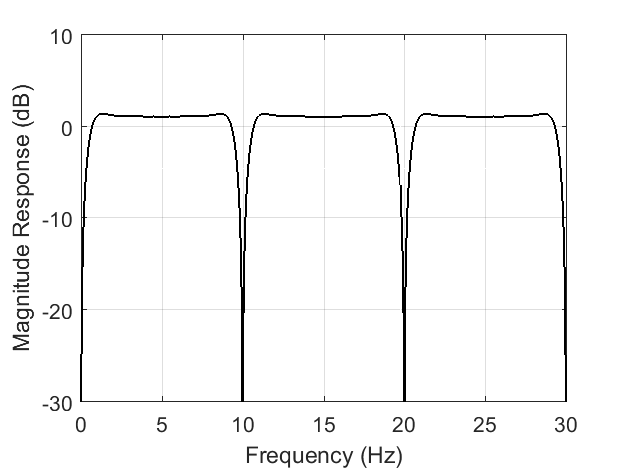
\includegraphics[width=\textwidth]{img/causal/mag_gauss.png}
        \caption{Gaussian~$\tau=3$}\label{fig:GaussKernel}
    \end{subfigure}
    \caption{Exemplary Causal Kernels}\label{fig:ExemplaryCausalKernels}
\end{figure}

As you can see from figure~\ref{fig:ExemplaryCausalKernels}, the (numerically calculated) magnitude responses of the four approaches are highly similar. Their key characteristic is the strong supression of the target frequency and its integer multiples.
Yet, note the difference in passbands. We find strong ringing in the passband for the uniform~(\ref{fig:UniformKernel}) and linear kernel~(\ref{fig:LinearKernel}), especially compared to the smooth transitions of the exponential~(\ref{fig:ExponentialKernel}) or Gaussian kernel~(\ref{fig:GaussKernel}).

\subsubsection{Exemplary Kernel Tuning}

We constructed a set of exponential kernels constructed with different $\tau$~\figref{fig:ExemplaryTauTuning} to explore their behavior.
We find it of note that that in the limiting case of $\tau = 0$, the exponential kernel virtually converges with the uniform kernel~\figref{fig:ExpTau0}. Using a $\tau$ equal to the artifacts period length, the exponential kernel almost fully converges with the simple comb filter~\figref{fig:ExpTau100}.
Note also that very high $\tau$ would return an impulse response, and therefore just pass all signals.

\begin{figure}[hbtp]
    \begin{subfigure}{.33\textwidth}
        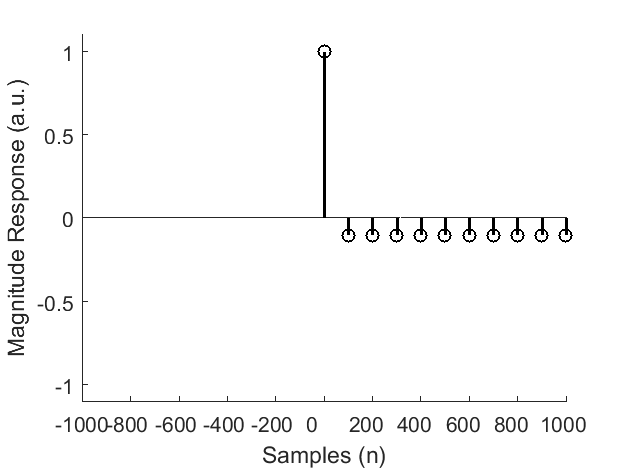
\includegraphics[width=\textwidth]{img/tau/kernel_exp_0.png}\\
        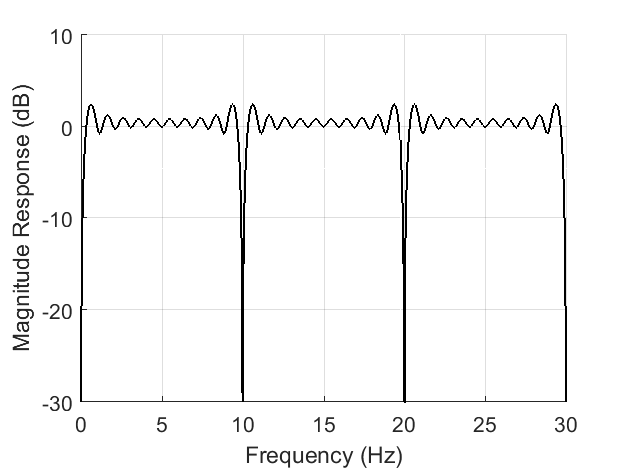
\includegraphics[width=\textwidth]{img/tau/mag_exp_0.png}
        \caption{Exponential~$\tau=0$}\label{fig:ExpTau0}
    \end{subfigure}
    \begin{subfigure}{.33\textwidth}
        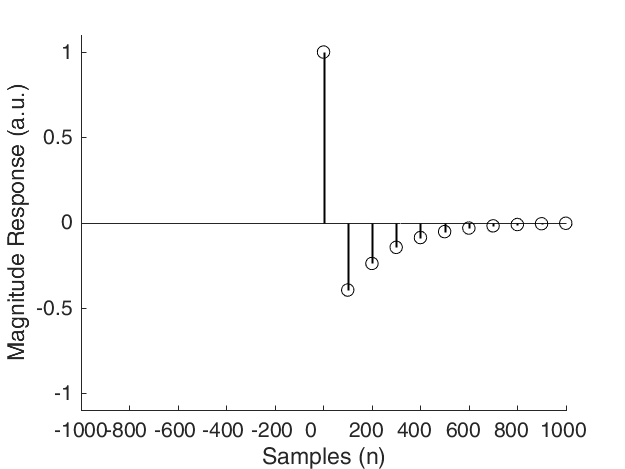
\includegraphics[width=\textwidth]{img/tau/kernel_exp_5.png}\\
        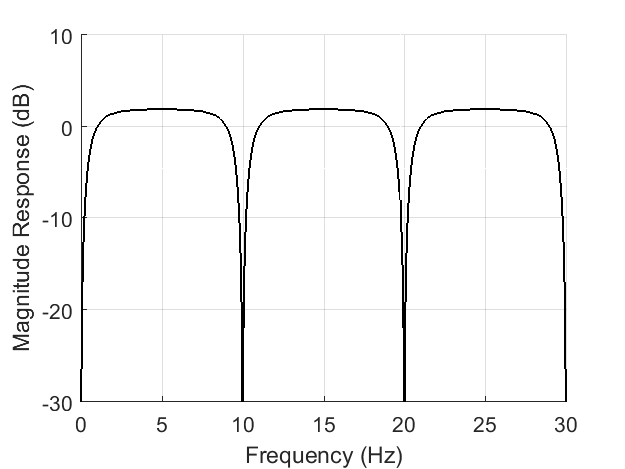
\includegraphics[width=\textwidth]{img/tau/mag_exp_5.png}
        \caption{Exponential~$\tau=5$}\label{fig:ExpTau5}
    \end{subfigure}
    \begin{subfigure}{.33\textwidth}
        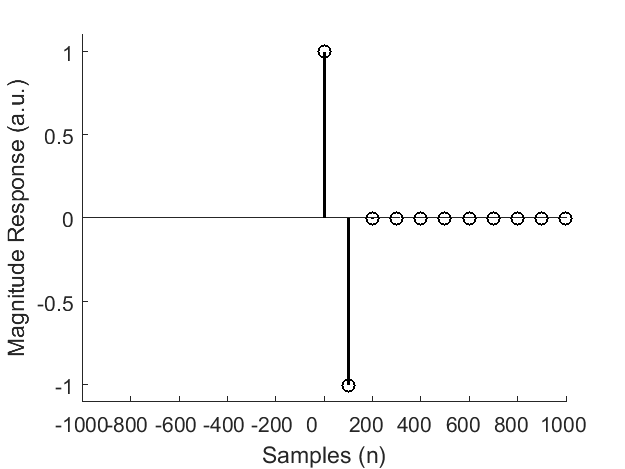
\includegraphics[width=\textwidth]{img/tau/kernel_exp_100.png}\\
        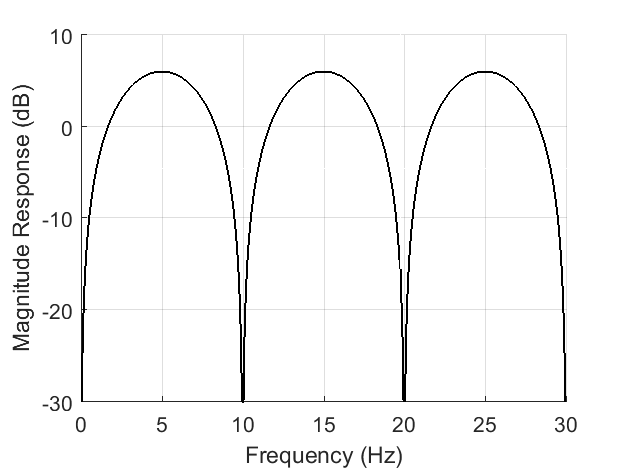
\includegraphics[width=\textwidth]{img/tau/mag_exp_100.png}
        \caption{Exponential~$\tau=100$}\label{fig:ExpTau100}
    \end{subfigure}
    \caption{Exemplary $\tau$ Tuning with $N=10$}\label{fig:ExemplaryTauTuning}
\end{figure}

Examine the following exponential kernels $N$~\figref{fig:ExemplaryNPTuning}.In the limiting case of $N = 1$, we acquire the simple comb filter~\figref{fig:ExNP1}. By increasing $N$ we achieve a flattening of the pass-band gain~\figref{fig:ExpNP50}.

\begin{figure}[hbtp]
    \begin{subfigure}{.33\textwidth}
        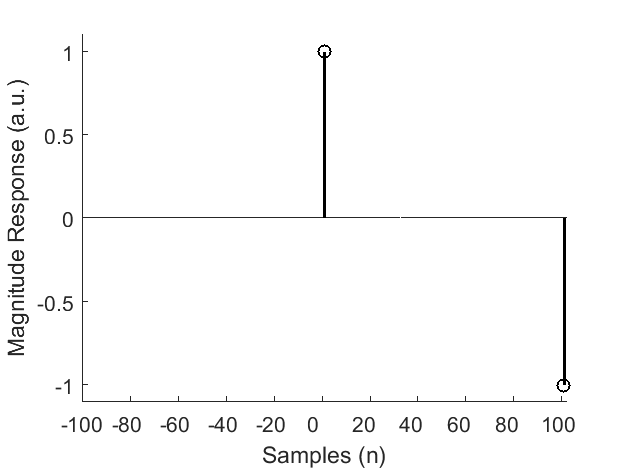
\includegraphics[width=\textwidth]{img/np/kernel_exp_1.png}\\
        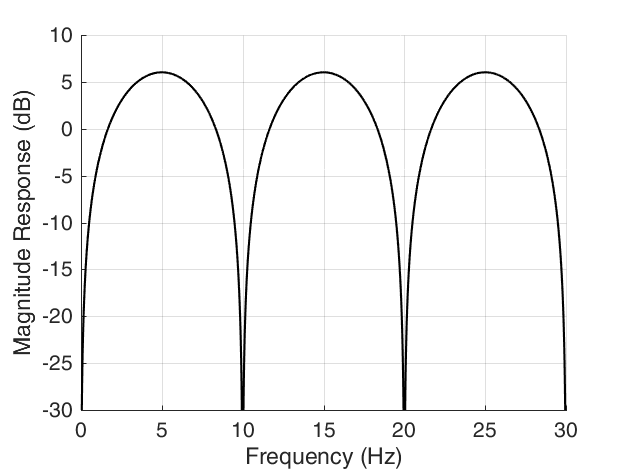
\includegraphics[width=\textwidth]{img/np/mag_exp_1.png}
        \caption{Exponential~$N=1$}\label{fig:ExNP1}
    \end{subfigure}
    \begin{subfigure}{.33\textwidth}
        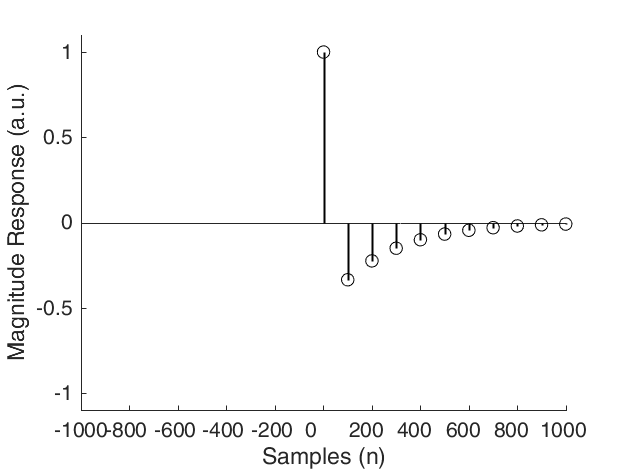
\includegraphics[width=\textwidth]{img/np/kernel_exp_10.png}\\
        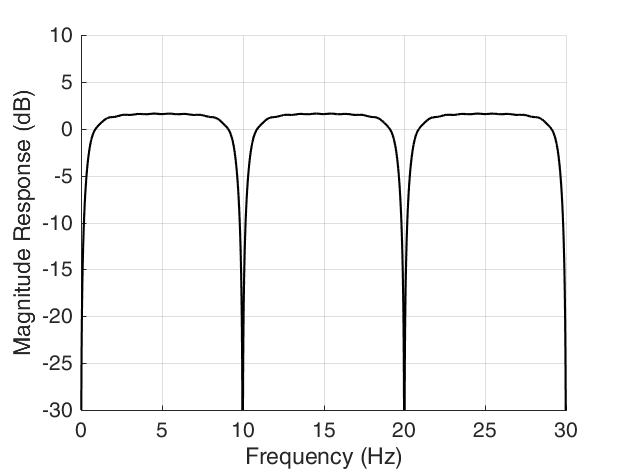
\includegraphics[width=\textwidth]{img/np/mag_exp_10.png}
        \caption{Exponential~$N=5$}\label{fig:ExpNP10}
    \end{subfigure}
    \begin{subfigure}{.33\textwidth}
        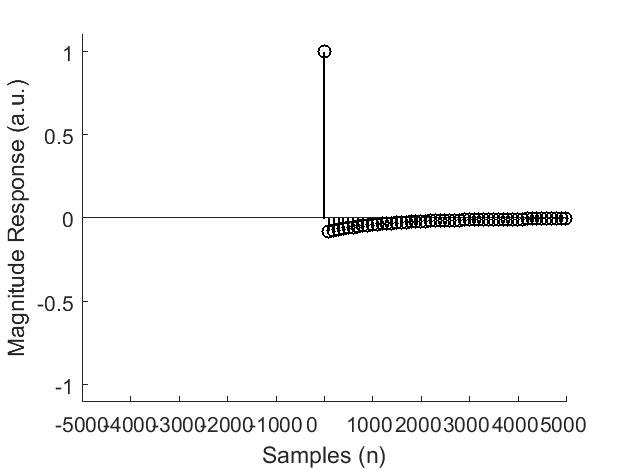
\includegraphics[width=\textwidth]{img/np/kernel_exp_50.png}\\
        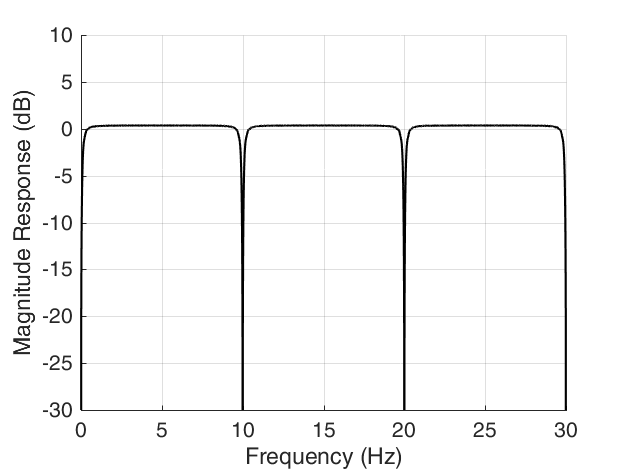
\includegraphics[width=\textwidth]{img/np/mag_exp_50.png}
        \caption{Exponential~$N=50$}\label{fig:ExpNP50}
    \end{subfigure}
    \caption{Exemplary $N$ Tuning with $\tau = 4$}\label{fig:ExemplaryNPTuning}
\end{figure}


\subsection{Evaluation on Simulated Signals}\label{sec:EvaluationSimulated}

To evaluate the filters, we tested them on simulated signals. The simulated signal was created as superposition of a 10 Hz \gls{tacs}-artifact, and an \gls{erp}.

\subsubsection{Simulation Parameters}

The \gls{erp} was simulated as numerical gradient of a flat top window, with amplitude set to 2 and a duration of 50 samples.

The amplitude of the artifact was simulated as a distorted, non-stationary semi-sinusoidal.
To achieve this, we distorted a sinusoidal by adding periodic white noise. Additionally, we had its amplitude driven by an Ornstein–Uhlenbeck, i.e. AR (1), process with mean 20, stiffness 0.5 and a variablity of 1, and an event-induced modulation with random phase and an amplitude of 1 over a Hanning window of 500 samples duration.

In that way, we were able to simulate event-independent modulations of the artifacts amplitude, and modulations locked to an event, as described by \citep{Noury_2016}, and which have a strong potential to mask any true event-related neurophysiological activity.

\subsubsection{Evaluation}

Subsequently, we explored different filter approaches, i.e.\ the two times four causal and symmetric weighted comb filters, all with a period number of 10. Additionally we evaluated adaptive discrete fourier filtering with the same period length of 10, and a linear regression of the artifact based on a copy of the efferent stimulation signal, as one could acquire from the \gls{tacs}-stimulator, e.g.\ the NeuroConn DC Plus.\footnote{Code can be found at \url{https://github.com/agricolab/ARtACS}}

We simulated 500 simulated trials, calculated the r² value based on the correlation of the filtered signal with the original \gls{erp} and performed a kernel density estimation of their distribution.

\begin{figure}[hbtp]
    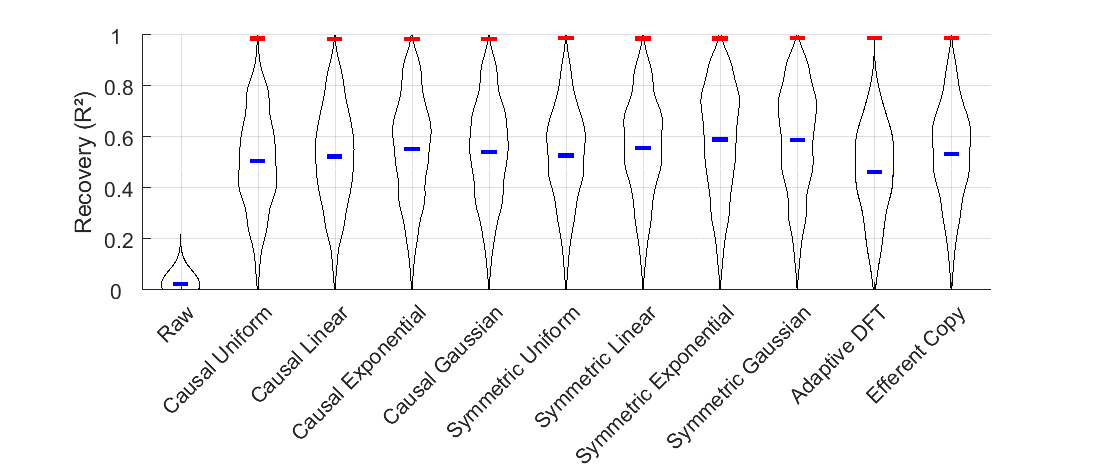
\includegraphics[width=\textwidth]{img/eva/recovery_erp.png}
    \caption{Figure shows the kernel density estimate of the R² between filtered and true signal, for several filter approaches. Blue bars indicate the mean, and red bars a robust estimate of the mode.}\label{fig:EvalOnErp}
\end{figure}

\subsection{Evaluation on real data}\label{sec:EvaluationData}

\section{Conclusion}

One approach to model such a unknown dynamical system is with a Lévy-process. The key characteristics of such a process is that it is governed by randomness of the change between time-points. The increments are independent from each other, and are sampled from a continuous probability distribution with is stationary for the whole duration of the process. In that framework, the uncertainty of the estimate changes as a function of lag. Consider furthermore that we we only consider

Ornstein-Uhlenbeck-Prozess discrete time AR (1) process

\begin{equation}
    a(t+1) = a(t) + \theta(\mu-a(t)) + e(t+1)
\end{equation}
where $\left|\theta\right|<1$ and $\mu$ is the model mean.
Note that if the stochastic process is skewed or has a non-zero expectation value, the filter might need to add a constant for debiasing the estimation. If the stochastic process allows for jumps, small $N$ might return a more reliable estimation than large $N$.

Negative weights
This paper only dicusses real filter weights real, but complex weights might be a solution to tackle artifacts with periods that are not integer divisibles of the sampling frequency.

\bibliographystyle{apalike-oadoi}
\bibliography{sample}

\end{document}
